%!TEX root = ../../../super_main.tex

\section{Consistent Pictograms}
\label{sec:consistent_pictograms}

Throughout this section the word \textit{pictogram} will be used to refer to an image (fetched from the set of all pictograms-imaged), however this image may also represent other levels of abstraction, for instance categories, profile pictures, sequences etc.
\\\\
Several pictograms will have to be displayed on different occasions throughout the different \giraf applications. This is resulting in a problem, namely that the methods used to display pictograms are inconsistent. For instance, some applications displays pictograms without a black border, which is unwanted by the customers. Furthermore, different applications uses different methods of displaying the selection of pictograms. These two problem caused the users to be confused and unable to use the application in some cases. 
\\\\
Based on the above mentioned problems it was decided that a common component to display pictograms was needed. Because this component will be used in several different contexts it needs to be very generic. This sets some requirement for the component, seen below:

\begin{itemize}
	\item Show or hide a title below the pictogram
	\item Indicate weather the pictogram is selected or not using a consistent background-color
	\item Indicate that a pictogram is editable (the user pressed the pictogram to edit it)
	\item Load the pictograms on a background thread instead of GUI-thread 
	\item Display a fall-back image (\mono{Drawable}) in case that the provided pictogram is not set (\mono{null})
	\item Scale images that are non square (height $\neq$ width) so that the overall pictogram is square
\end{itemize}

A common component was then implemented based on the requirement above. Now, the different applications (including \ct) will have to update the way they display pictograms so that they now use this new component instead of whatever they did before. A screenshot from the Oasis application (user management) can be seen in \figref{fig:pictogram_component_use}. This application uses the component in two different ways, namely one for showing different departments in the institutions (seen on the left), using a fallback-image (since a department does not currently have an image associated), but they also use it for displaying the citizens in a given department (seen on the right). Please note that the application seen is still in development, and may not look like this at any point in the future. 

\begin{figure}[!htbp]
	\centering
	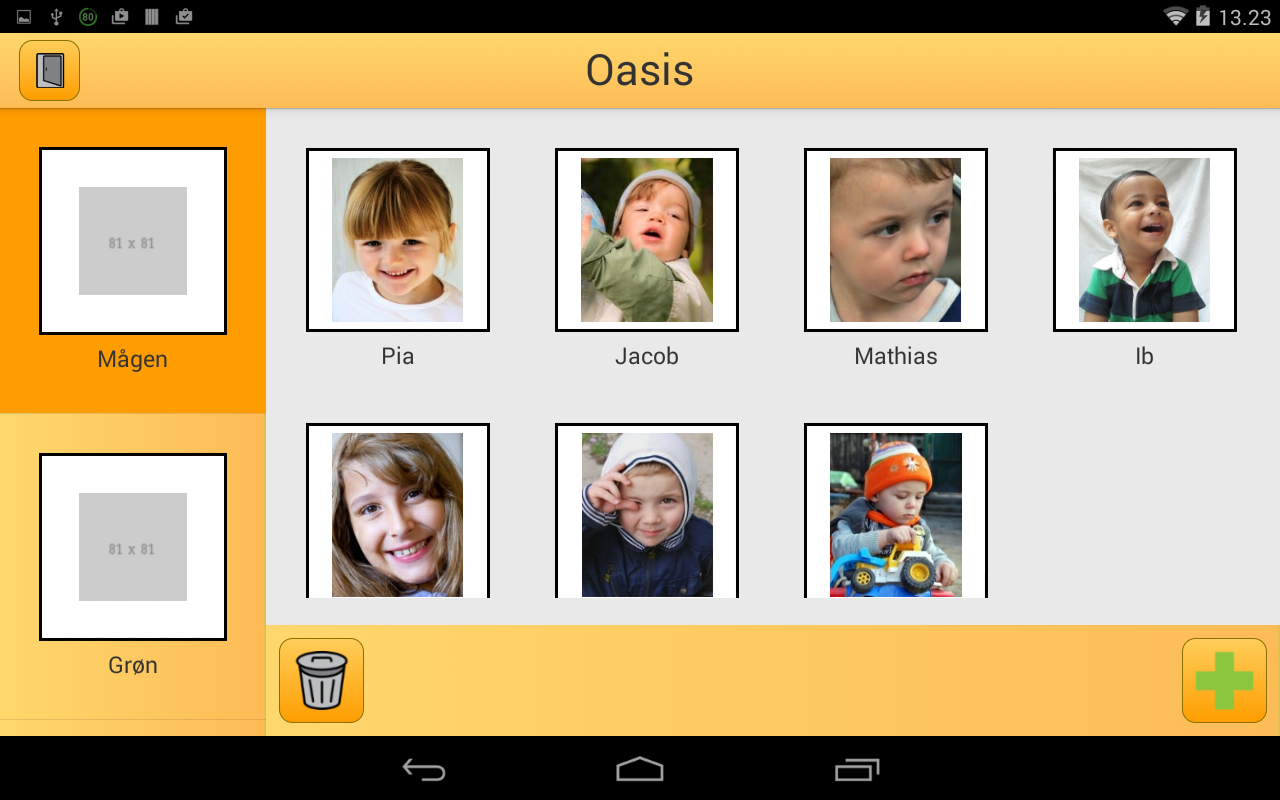
\includegraphics[width=\textwidth]{sprint_three/pictogram_component_use}
	\caption{Usage of pictogram component}
	\label{fig:pictogram_component_use}
\end{figure}